%%%%%%%%%%%%%%%%%%%%%%%%%%%%%%%%%%%%%%%%%
% Beamer Presentation
% LaTeX Template
% Version 1.0 (10/11/12)
%
% This template has been downloaded from:
% http://www.LaTeXTemplates.com
%
% License:
% CC BY-NC-SA 3.0 (http://creativecommons.org/licenses/by-nc-sa/3.0/)
%
%%%%%%%%%%%%%%%%%%%%%%%%%%%%%%%%%%%%%%%%%

%----------------------------------------------------------------------------------------
%	PACKAGES AND THEMES
%----------------------------------------------------------------------------------------

\documentclass{beamer}

\mode<presentation> {

% The Beamer class comes with a number of default slide themes
% which change the colors and layouts of slides. Below this is a list
% of all the themes, uncomment each in turn to see what they look like.

% \usetheme{default}
%\usetheme{AnnArbor}
%\usetheme{Antibes}
%\usetheme{Bergen}
% \usetheme{Berkeley}
%\usetheme{Berlin}
%\usetheme{Boadilla}
%\usetheme{CambridgeUS}
%\usetheme{Copenhagen}
%\usetheme{Darmstadt}
%\usetheme{Dresden}
%\usetheme{Frankfurt}
%\usetheme{Goettingen}
%\usetheme{Hannover}
%\usetheme{Ilmenau}
%\usetheme{JuanLesPins}
%\usetheme{Luebeck}
%\usetheme{Madrid}
%\usetheme{Malmoe}
%\usetheme{Marburg}
%\usetheme{Montpellier}
%\usetheme{PaloAlto}
%\usetheme{Pittsburgh}
%\usetheme{Rochester}
%\usetheme{Singapore}
%\usetheme{Szeged}
%\usetheme{Warsaw}

% As well as themes, the Beamer class has a number of color themes
% for any slide theme. Uncomment each of these in turn to see how it
% changes the colors of your current slide theme.

%\usecolortheme{albatross}
%\usecolortheme{beaver}
%\usecolortheme{beetle}
%\usecolortheme{crane}
%\usecolortheme{dolphin}
%\usecolortheme{dove}
%\usecolortheme{fly}
%\usecolortheme{lily}
%\usecolortheme{orchid}
%\usecolortheme{rose}
%\usecolortheme{seagull}
%\usecolortheme{seahorse}
%\usecolortheme{whale}
%\usecolortheme{wolverine}

%\setbeamertemplate{footline} % To remove the footer line in all slides uncomment this line
%\setbeamertemplate{footline}[page number] % To replace the footer
%line in all slides with a simple slide count uncomment this line

%\setbeamertemplate{navigation symbols}{} % To remove the navigation
%symbols from the bottom of all slides uncomment this line
}
%% \usepackage[dvipsnames]{xcolor}
\usepackage{graphicx} % Allows including images
\usepackage{booktabs} % Allows the use of \toprule, \midrule and \bottomrule
                      % in tables
%% \usepackage{color}
\usepackage[utf8x]{inputenc}
\usepackage{lmodern,textcomp}

\DeclareGraphicsExtensions{.pdf,.png,.jpg}
\graphicspath{{../../papers/FX/}}
\usepackage{amssymb,amsmath,amsthm,amsfonts}
\usepackage{mathrsfs}
\usepackage{dsfont}
\usepackage{enumerate}

%\newtheorem{mdef}{Definition}
%\newtheorem{theorem}{Theorem}
\newcommand{\eqsplit}[2]{
  \begin{equation}\label{#2}
    \begin{split}
      #1
    \end{split}
  \end{equation}}
\newcommand{\eqnsplit}[1]{
  \begin{eqnarray*}
    #1
  \end{eqnarray*}}
\newcommand{\tran}[1]{
  \tilde{#1}
}
\newcommand{\td}[2]{
  \frac{d #1}{d #2}
}
\newcommand{\pd}[2]{
  \frac{\partial #1}{\partial #2}
}
\newcommand{\ppd}[2]{
  \frac{\partial^2 #1}{\partial #2^2}
}
\newcommand{\pdd}[3]{
  \frac{\partial^2 #1}{\partial #2 \partial #3}
}
\newcommand{\otd}[1]{
  \frac{d}{d #1}
}
\newcommand{\opd}[1]{
  \frac{\partial}{\partial #1}
}
\newcommand{\oppd}[1]{
  \frac{\partial^2}{\partial #1^2}
}
\newcommand{\opdd}[2]{
  \frac{\partial^2}{\partial #1 \partial #2}
}
\newcommand{\ket}[1]{
  |#1\rangle
}
\newcommand{\bra}[1]{
  \langle#1|
}
\newcommand{\inn}[1]{
  \langle#1\rangle
}
\newcommand{\mean}[1]{
  \langle#1\rangle
}
\newcommand{\tr}{
  \text{tr}\,
}
\newcommand{\re}{
  \text{Re}\,
}
\newcommand\im{
  \text{Im}\,
}
\newcommand{\var}{
  \text{var}
}
\newcommand{\arcsinh}{
  \sinh^{-1}
}
\newcommand{\arccosh}{
  \cosh^{-1}
}
\newcommand{\erfc}{
  \text{erfc}
}
\newcommand{\E}{
  \mathbb{E}
}
\renewcommand{\P}{
  \mathbb{P}
}
\newcommand{\I}[1]{
  \mathbf{1}_{\{#1\}}
}
\newcommand{\1}[1]{
  \mathds{1}_{\{#1\}}
}
\newcommand{\diag}{
  \text{diag\,}
}
\newcommand{\M}{
  {\text{max}}
}
\newcommand{\m}{
  {\text{min}}
}
\newcommand{\ph}{
  {\text{arg}\,}
}
\newcommand\erf{
  \text{erf}
}
\renewcommand\vec[1]{
  \mathbf{#1}
}
\newcommand\mtx[1]{
  \mathbf{#1}
}
\newcommand\ed{
  \,{\buildrel d \over =}\,
}




%----------------------------------------------------------------------------------------
%	TITLE PAGE
%----------------------------------------------------------------------------------------
\title{Do return series have power-law tails with the same index?}
% The short title appears at the bottom of
% every slide, the full title is only
% on the title page

\author{Thomas Mikosch, Casper de Vries, Xie Xiaolei} % Your name
\institute[UCPH] % Your institution as it will appear on the bottom of every slide, may be shorthand to save space
{
University of Copenhagen \\ % Your institution for the title page
\medskip
\textit{xie@math.ku.dk} % Your email address
}
\date{\today} % Date, can be changed to a custom date

\begin{document}

\begin{frame}
\titlepage % Print the title page as the first slide
\end{frame}

% \begin{frame}
% \frametitle{Overview}
% \tableofcontents
% \end{frame}

%----------------------------------------------------------------------------------------
%	PRESENTATION SLIDES
%----------------------------------------------------------------------------------------
% \section{Simple dependence models}
%------------------------------------------------
\begin{frame}
  \frametitle{Questions that we want to answer}
  \textcolor[HTML]{990033}{\bf We know}

  If assumed stationary, equity return series are often seen to be
  heavy-tailed -- a stylized fact of econometrics.
  
  \textcolor[HTML]{990033}{\bf But}
  \begin{itemize}
    \item Given the wide confidence bands of estimated tail indices,
      are they actually the same?
    \item Are tail parameters of different equity return series in the same
      market related to each other?
    \item How are investors' preferences over an equity affected by
      tail parameters?
  \end{itemize}
\end{frame}

\begin{frame}
  \frametitle{Motivation}
  \begin{itemize}
  \item Curiosity
    \item Many multivariate GARCH processes have a stationary
      distribution with power-law tails:
      \begin{enumerate}
        \item CCC-GARCH of Bollerslev \cite{bollerslev:1990} and
          Jeantheau \cite{jeantheau:1998}.
        \item Orthogonal GARCH of
          Alexander and Chibumba \cite{alexander:chibumba:1996},
        \item GO-GARCH by van der Weide \cite{Weide2002} which
          generalizes Orthogonal GARCH.
        \item Full Factor GARCH of Vrontos et
          al. \cite{vrontos2003full}
        \item Generalized Orthogonal Factor GARCH of Lanne and
          Saikkonen  \cite{lanne2007modelling}
      \end{enumerate}
  \end{itemize}
\end{frame}


\begin{frame}
  \frametitle{CCC-GARCH, Kesten's theorem \& power-law tail}
  A 2D CCC-GARCH model reads
  \begin{eqnarray*}
    \begin{pmatrix}
      \sigma_{1, t}^2 \\
      \sigma_{2, t}^2
    \end{pmatrix}
    &=&
    \begin{pmatrix}
      \alpha_{1, 1} & \alpha_{1, 2} \\
      \alpha_{2, 1} & \alpha_{2, 2} \\
    \end{pmatrix}
    \begin{pmatrix}
      X_{1, t-1}^2 \\
      X_{2, t-1}^2
    \end{pmatrix}
    +
    \begin{pmatrix}
      \beta_{1, 1} & \beta_{1, 2} \\
      \beta_{2, 1} & \beta_{2, 2} \\
    \end{pmatrix}
    \begin{pmatrix}
      \sigma_{1,t-1}^2 \\
      \sigma_{2,t-1}^2 \\
    \end{pmatrix}
    +
    \begin{pmatrix}
      \omega_1 \\
      \omega_2
    \end{pmatrix} \\
    &=&
    \underbrace{
      \begin{pmatrix}
        \alpha_{1,1} Z_{1,t-1}^2 + \beta_{1,1} & \alpha_{1,2} Z_{2,t-1}^2 + \beta_{1,2} \\
        \alpha_{2,1} Z_{1,t-1}^2 + \beta_{2,1} & \alpha_{2,2} Z_{2,t-1}^2 + \beta_{2,2}
      \end{pmatrix}
    }_{A_t}
    \underbrace{
      \begin{pmatrix}
        \sigma_{1,t-1}^2 \\
        \sigma_{2,t-1}^2
      \end{pmatrix}
    }_{Y_{t-1}}
    +
    \underbrace{
      \begin{pmatrix}
        \omega_1 \\
        \omega_2
      \end{pmatrix}
    }_{B}
  \end{eqnarray*}
  where $X_{1, t}, X_{2, t}$ are return series, whose conditional
  variances are $\sigma_{1, t}^2, \sigma_{2, t}^2$.
  When $\forall i,j, \alpha_{i, j} > 0, \beta_{i,j} > 0$ and certain
  conditions are satisfied, Kesten's theory \cite{kesten:1973} gives
  \[
  \lim_{u \to \infty} u^{\alpha}
  \P(\inn{\vec v, Y} > u) = e_\alpha(\vec v)
  \]
  where $e_\alpha(\cdot): \sphere^{1} \to \reals_+$.
  {\bf Each component of $Y_t$ shares the same tail index $\alpha$}.
  
\end{frame}

\begin{frame}
  \frametitle{Heavy-tailedness of equity returns}
  \begin{minipage}[t]{0.5\linewidth}
    \begin{figure}[htb!]
      \begin{minipage}{1.0\linewidth}
        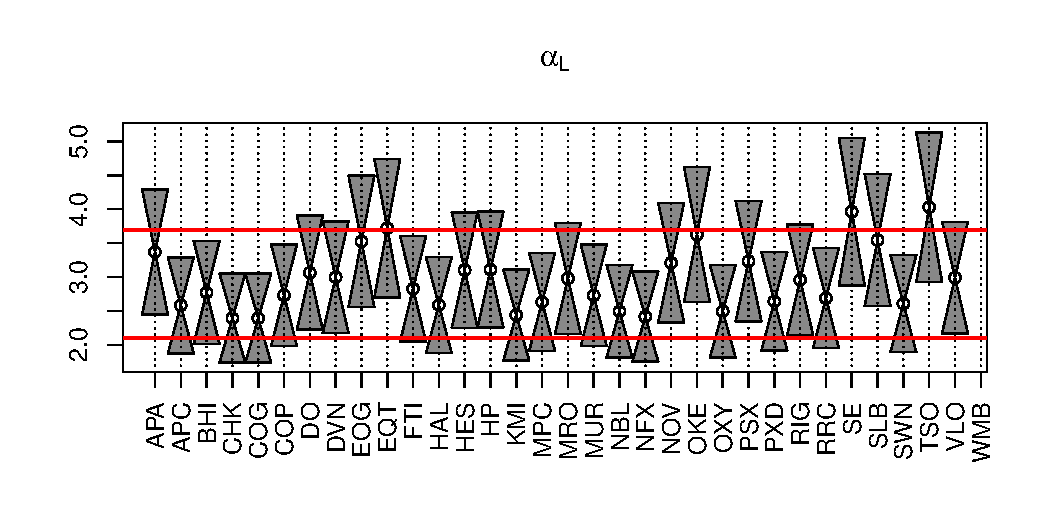
\includegraphics[width=\textwidth, trim={0, 0.8cm, 0, 2cm}, clip]
                        {Energy_lower.pdf}
      \end{minipage}
      \begin{minipage}{1.0\linewidth}
        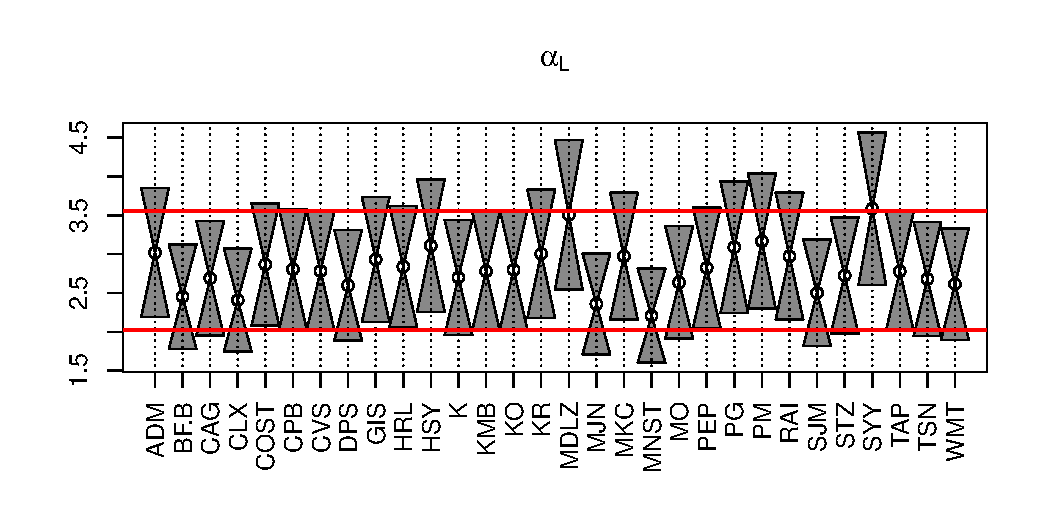
\includegraphics[width=\textwidth, trim={0, 0.8cm, 0, 2cm}, clip]
                        {Consumer_Staples_lower.pdf}
      \end{minipage}
      \begin{minipage}{1.0\linewidth}
        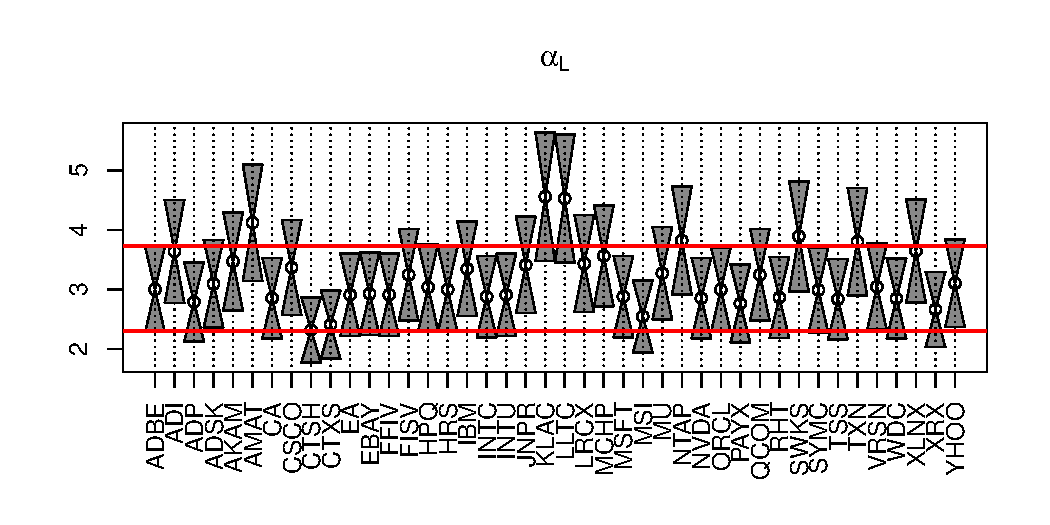
\includegraphics[width=\textwidth, trim={0, 0.8cm, 0, 2cm}, clip]
                        {Information_Technology_lower.pdf}
      \end{minipage}
      \caption{\tiny Hill estimates daily return series in
        sectors of the S\&P 500 index. The data span  from 1 January
        2010 to 31 December 2014 and comprise $n=1304$ observations.
        The graphs from top to bottom correspond to the ``Energy'',
        ``Consumer Staples'' and ``Information Technology'' sectors.
      }\label{fig:1}
    \end{figure}
  \end{minipage}\hfill
  \begin{minipage}[t]{0.5\linewidth}
    \textcolor[HTML]{990033}{\bf Interesting observations}
    \begin{itemize}
      \item Hill estimates of equity tail indices are often found
        between 2.5 $\sim$ 4.5
      \item The estimates are contained within each other's confidence bands
      \item Different sectors have different levels of variability in
        the tail indices.
    \end{itemize}
  \end{minipage}
\end{frame}

\begin{frame}
  \frametitle{Test for equal tail index: using Hill estimator}
  \begin{itemize}
    \item   Two return series $X_1, X_2, \dots, X_n$ and
      $Y_1, Y_2, \dots, Y_n$, with lower-tail indices
      $\alpha_X$ and $\alpha_Y$.
    \item We want to test the null hypothesis $H_0: \alpha_X = \alpha_Y$.
  \end{itemize}
  Under $H_0$, we have
  \[
  \sqrt k [\hat \alpha_X(k) - \hat \alpha_Y(k)] \overset{d}{\to}
  N(0, \alpha_X^2 + \alpha_Y^2)
  \]
  $\hat \alpha_X(k)$: Hill estimate of $\alpha_X$ using $k$ upper
  order statistics.
\end{frame}

\begin{frame}
  \frametitle{\small Test for equal tail index: testing for a
    changed extreme quantile}
  Given a series $X_1, X_2, \dots, X_n$ where $X_i \sim F_i$, Hoga
  \cite{hoga:2016} proposed a test for the hypothesis $H_0$:
  $1 < \exists k < n$ such that
  \begin{itemize}
    \item $F_i^{-1}(1 - p) = F_j^{-1}(1 - p)$, for all $1 \leq i < j < k$
    \item $F_{k-1}^{-1}(1 - p) \neq F_k^{-1}(1 - p)$ and
      $F_i^{-1}(1-p) = F_k^{-1}(1-p)$ for all $i \geq k$.
  \end{itemize}
  where $p = p_n \to 0$ as $n \to \infty$. The test statistic is
  \begin{tiny}
  \[
  T_n = \sup_{s \in [t_0, 1 - t_0]}
  \dfrac{  \big[s (1 - s) \log \big(\hat x_p(0, s)/\hat x_p(s, 1)\big)
      \big]^2}{
    \int_{t_0}^s\big[r \log \big( \hat x_p(0, r)/\hat x_p(0, s)
      \big)
      \big]^2 dr
    +
    \int_{s}^{1 - t_0}
    \big[
      (1 - r) \log \big(
      \hat x_p(r, 1)/
      \hat x_p(s, 1)
      \big)
      \big]^2 dr}
  \]
  \end{tiny}
  where
  \begin{small}
  \[
  \hat x_p(s, t) = X_{k, s, t}
  \left({n p \over k}\right)^{-1/{\hat \alpha}}
  \]
  \begin{itemize}
    \item $X_{k, s, t}$ is the $k$-th largest value among
      $X_{\floor{n s} + 1}, \dots, X_{\floor{n t}}$.
    \item   The {\bf asymptotic distribution of $T_n$ under $H_0$ is not
      available} explicitly, but given as the distribution of a
      function of a standard Brownian motion -- Computed by simulation.
  \end{itemize}
  \end{small}
\end{frame}

\begin{frame}
  \frametitle{Results of the tests on S\&P 500 sectors}
\begin{figure}[htb!]
  \begin{minipage}{0.33\linewidth}
    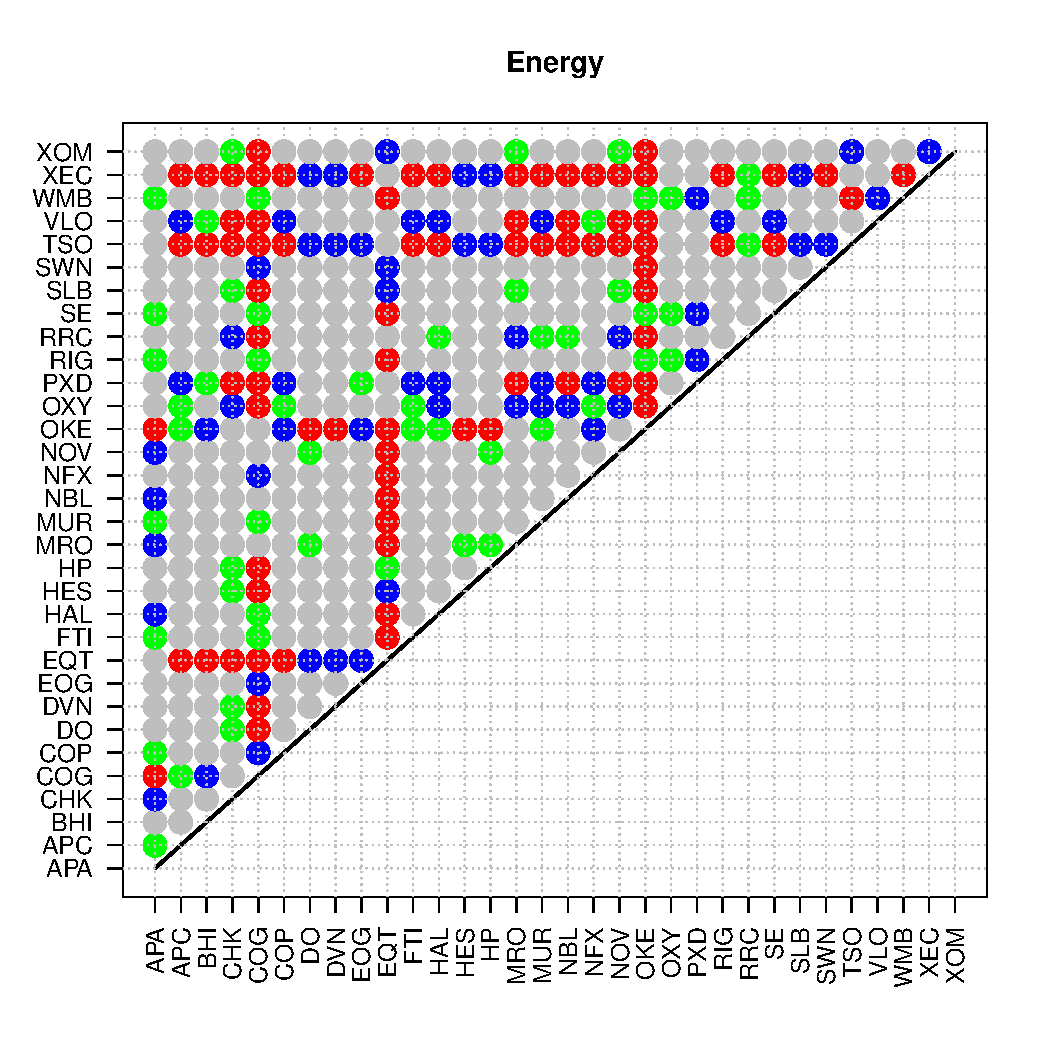
\includegraphics[
      width=\textwidth,
      trim={0.3cm, 0.8cm, 1cm, 0.6cm}, clip
    ]{HillTest_Energy.pdf}
  \end{minipage}\hfill
  \begin{minipage}{0.33\linewidth}
    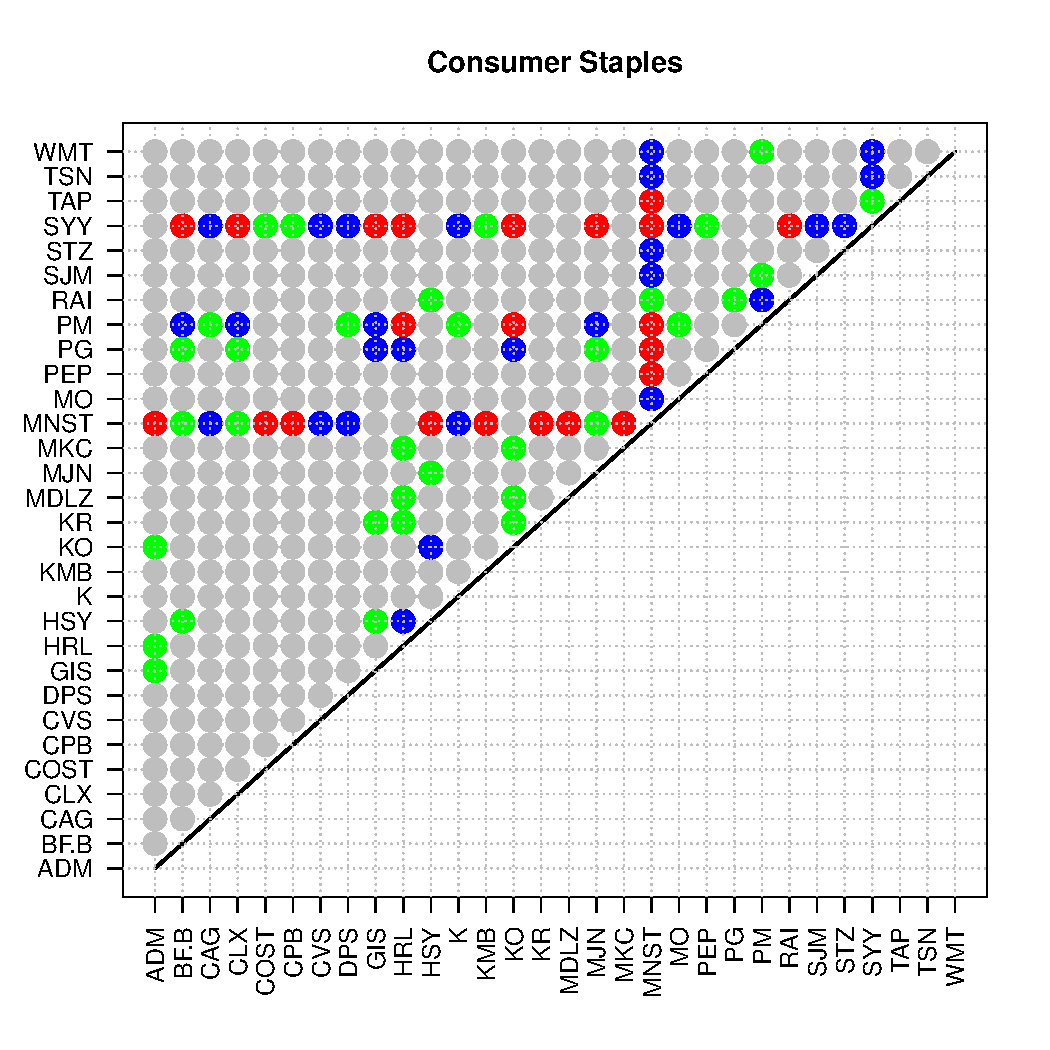
\includegraphics[
      width=\textwidth,
      trim={0.3cm, 0.8cm, 1cm, 0.6cm}, clip
    ]{HillTest_CS.pdf}
  \end{minipage}\hfill
  \begin{minipage}{0.33\linewidth}
    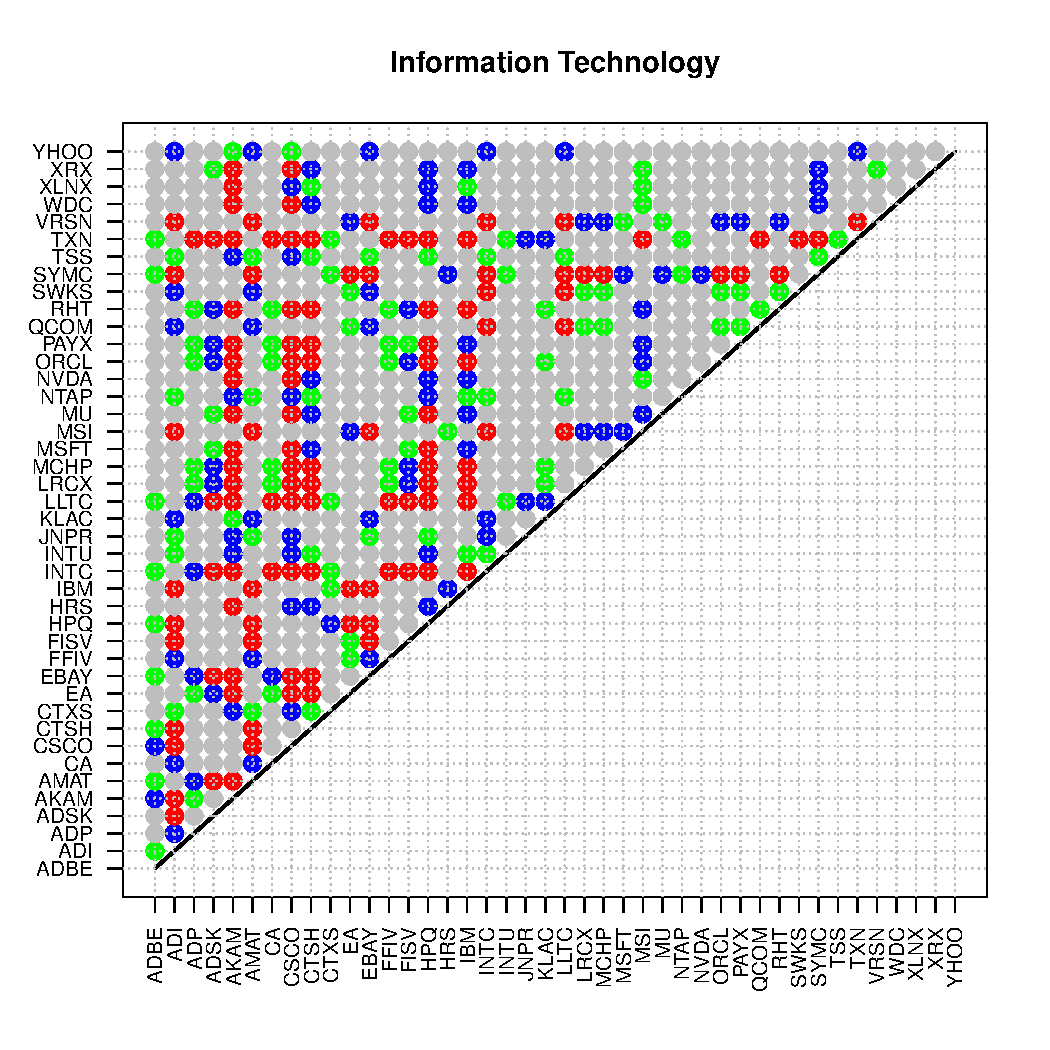
\includegraphics[
      width=\textwidth,
      trim={0.3cm, 0.8cm, 1cm, 0.6cm}, clip
    ]{HillTest_IT.pdf}
  \end{minipage}
  \begin{minipage}{0.33\linewidth}
    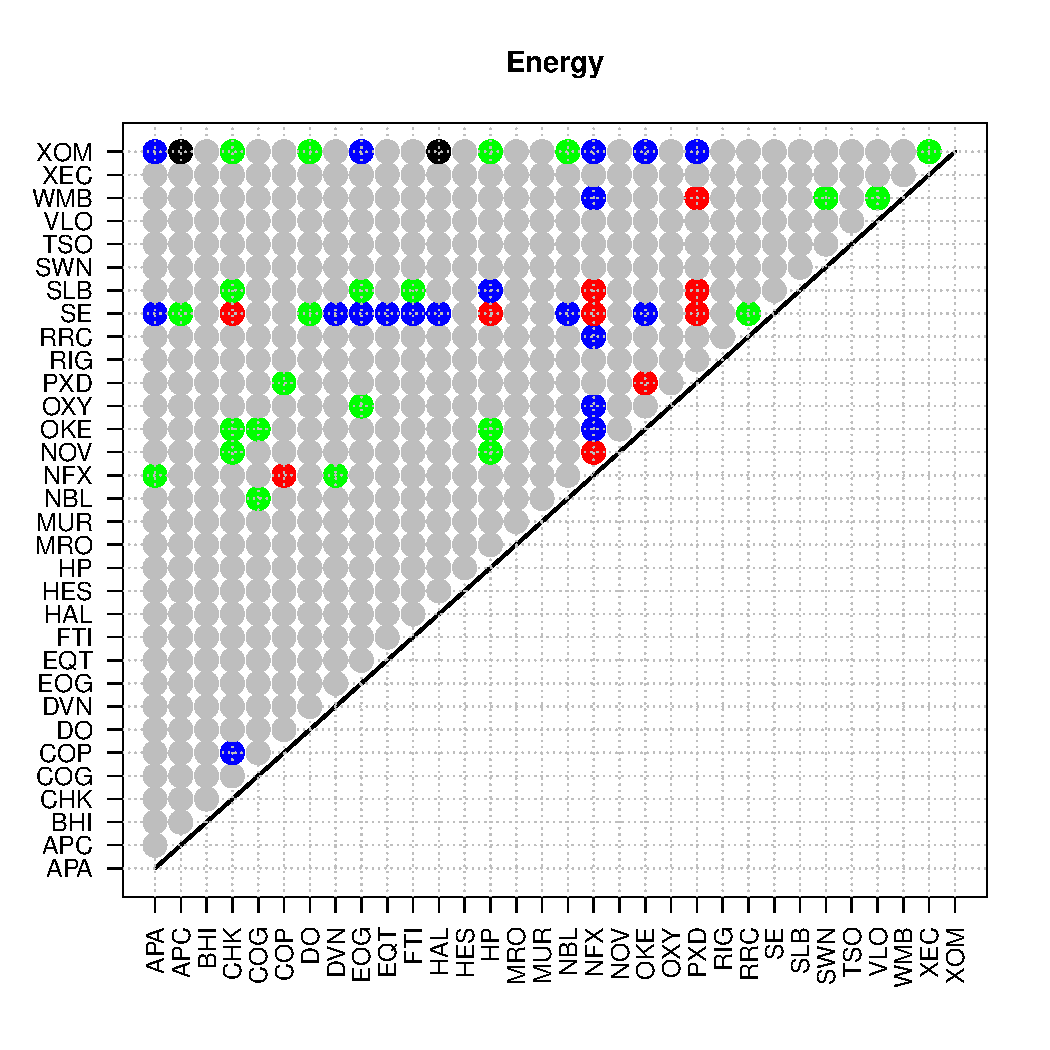
\includegraphics[
      width=\textwidth,
      trim={0.3cm, 0.8cm, 1cm, 0.6cm}, clip
    ]{Hoga_Energy_pair.pdf}
  \end{minipage}\hfill
  \begin{minipage}{0.33\linewidth}
    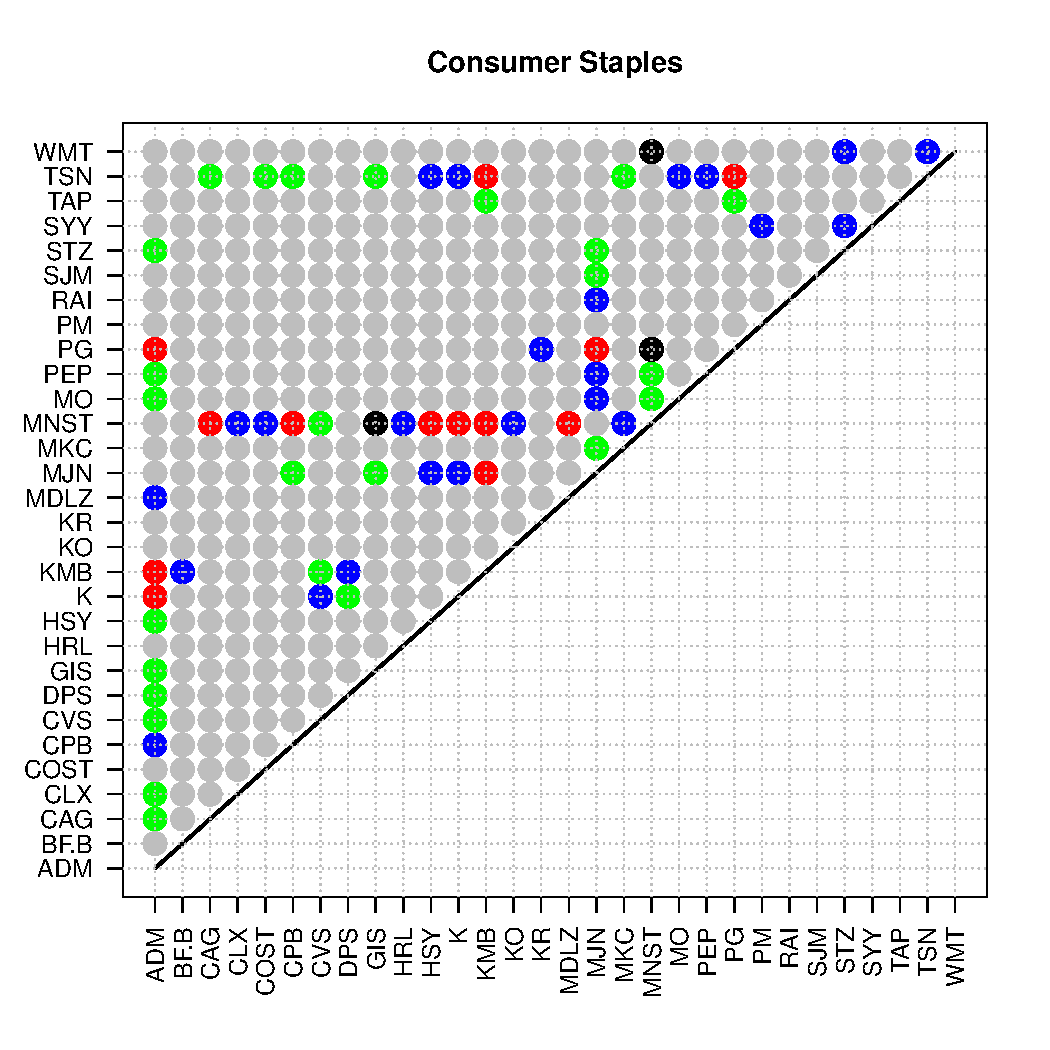
\includegraphics[
      width=\textwidth,
      trim={0.3cm, 0.8cm, 1cm, 0.6cm}, clip
    ]{Hoga_CS_pair.pdf}
  \end{minipage}\hfill
  \begin{minipage}{0.33\linewidth}
    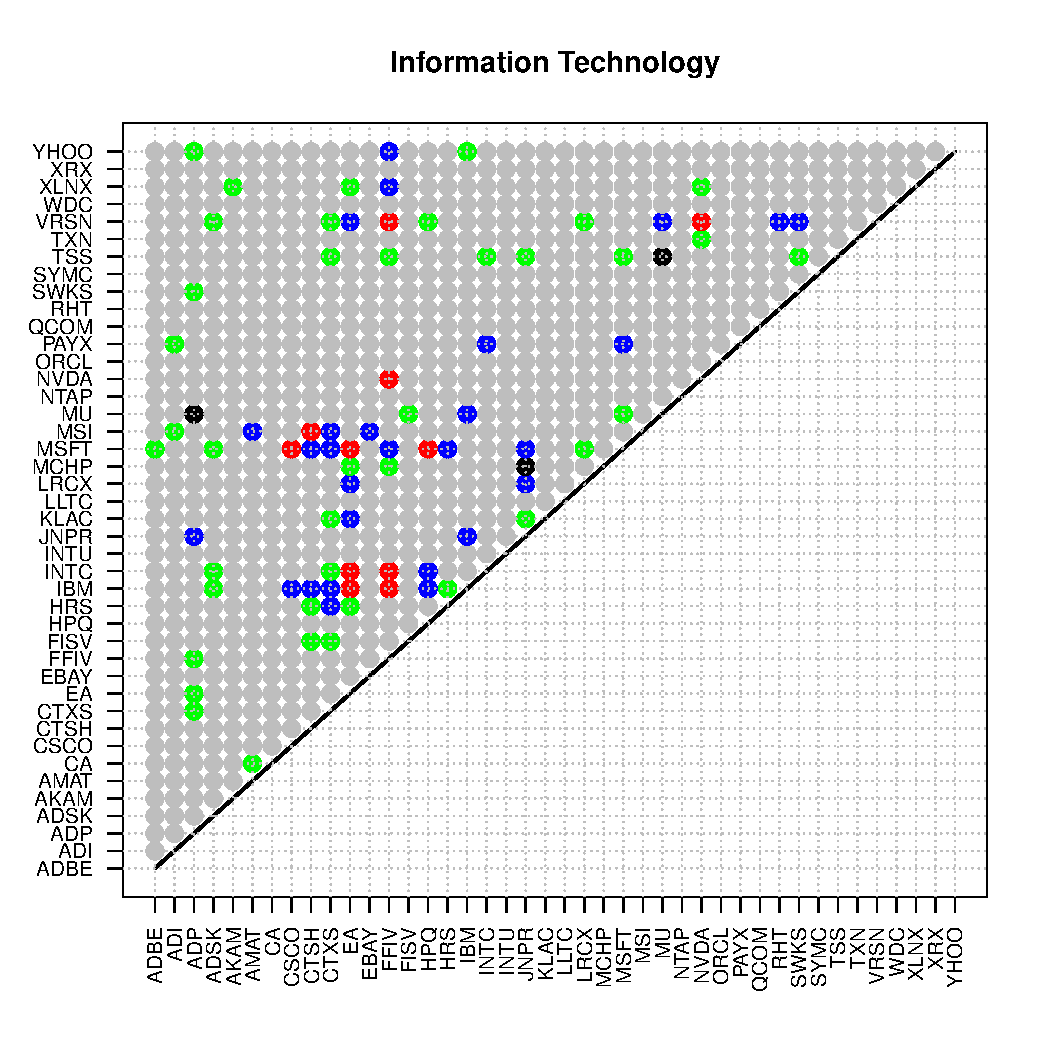
\includegraphics[
      width=\textwidth,
      trim={0.3cm, 0.8cm, 1cm, 0.6cm}, clip
    ]{Hoga_IT_pair.pdf}
  \end{minipage}
  \caption{\tiny
    {\em Top row}: Hill-based test.
    %% The test statistic in $\hat\alpha_X-\hat \alpha_Y$ is based
    %% on Hill estimates 
    %% of $\alpha_X$ and $\alpha_Y$. 
    The green, blue and red points correspond to pairs of stock in a sector
    when the test statistic is outside the intervals $[q_{0.075},q_{0.925}]$,
    $[q_{0.05},q_{0.95}]$,  $[q_{0.025},q_{0.975}]$
    %% $q_p$ is the $p$-quantile of the limiting 
    %% $N(0,\alpha_X^2+\alpha_Y^2)$-\ds\ of the test statistic in
    %% \eqref{eq:x1}. Grey points stand for pairs for which the test
    %% statistic is inside $[q_{0.075},q_{0.925}]$. 
    {\em Bottom row:} Hoga's test.
    The green, blue and red points correspond to pairs of stock in a sector 
    when the test statistic $T_n$ exceeds the $85\%$-, $90\%$-,
    $95\%$-quantile of the limit distribution .
  %% Grey points stand for pairs for which the test statistic is below
  %% the \asy\ $85\%$-quantile. Black points represent 
  %%   pairs for which the computation of $T_n$ fails for given precision  
  %%   requirements and time limits.
    The same number (50) of upper order statistics is used for both tests.}
  \label{fig:PairTest} 
\end{figure}
\end{frame}

\begin{frame}
  \frametitle{The scale parameter}
  Assume the equity return $X_t$ is stationary and follows Pareto
  distribution when $X < -K$:
  \[
  \P(X_t < -x) = {
    K^\alpha
    \over
    x^\alpha
  }, \quad x > K
  \]
  Hill's \cite{hill1975simple} maximum likelihood estimator for $K$ is
  \[
  \hat K_k = \left(
  {k \over n}
  \right)^{1/\hat \alpha_k} X_{(k)}
  \]
  where
  \begin{itemize}
  \item $n$ is the sample size
  \item $\hat \alpha_k$ is Hill's estimator of the tail index of $k$
    upper order statistics.
  \item $X_{(k)}$ is the $k$-th upper order statistic in the sample
  \end{itemize}
  By asymptotic normality of upper order statistics,
  \[
  \sqrt k (\hat K_k - K) \overset{d}{\to} N(0, K^2/\alpha^2)
  \]
\end{frame}

\begin{frame}
  \frametitle{Hill estimates of the scale parameter for S\&P 500
    sectors}
  {\scriptsize
  S\&P 500: Standard \& Poor's stock index. A weighted average of
  prices of 500 or so stocks listed on NYSE and NASDAQ. Stocks are
  grouped into 10 sectors. The \textcolor[HTML]{990033}{\bf Energy,
    Consumer Staples, IT} sectors are shown here.}
  \begin{minipage}{0.65\linewidth}
  \begin{figure}[htb!]
    \centering
    \begin{minipage}{0.33\linewidth}
      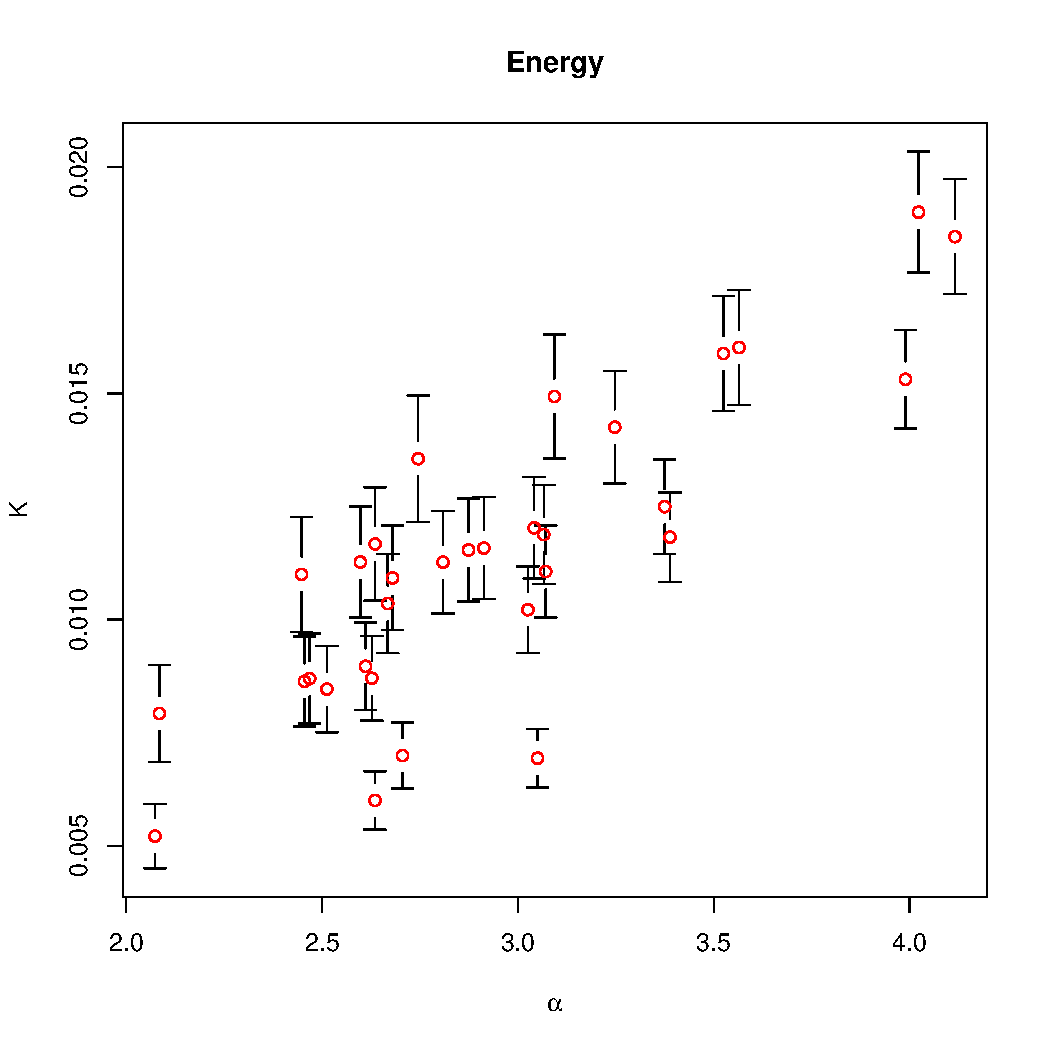
\includegraphics[width=\textwidth]
                      {Energy_K.pdf}
    \end{minipage}\hfill
    \begin{minipage}{0.33\linewidth}
      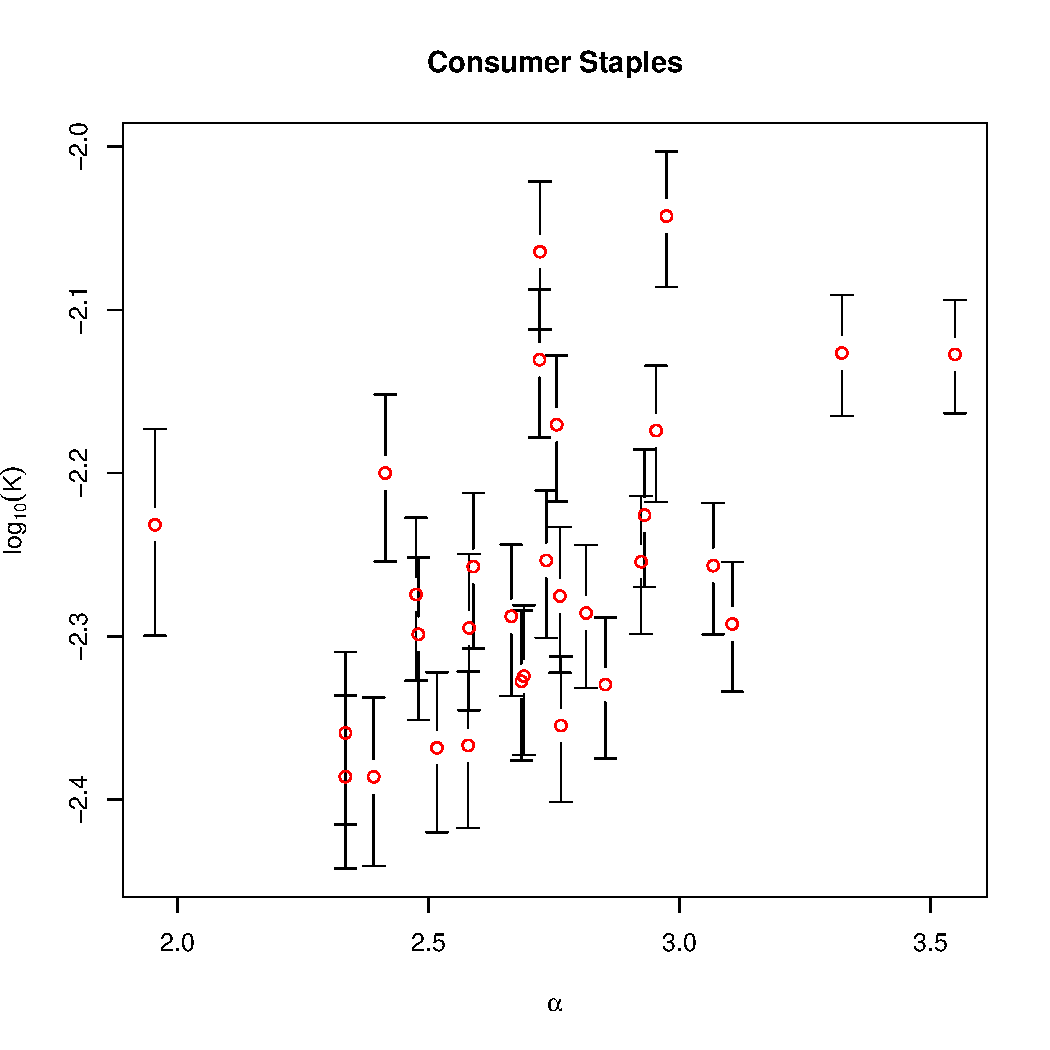
\includegraphics[width=\textwidth]
                      {CS_K.pdf}
    \end{minipage}\hfill
    \begin{minipage}{0.33\linewidth}
      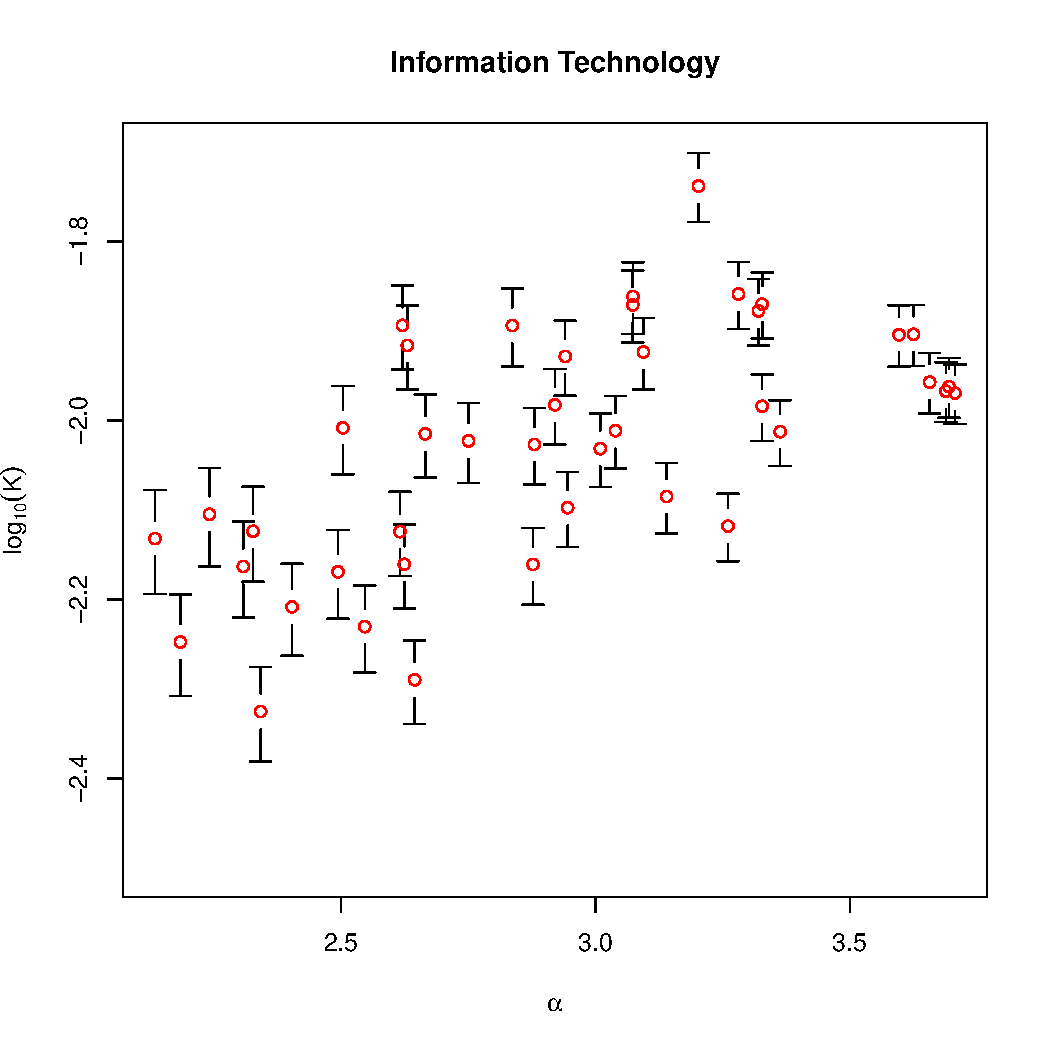
\includegraphics[width=\textwidth]
                      {IT_K.pdf}
    \end{minipage}
  \begin{minipage}{0.33\linewidth}
    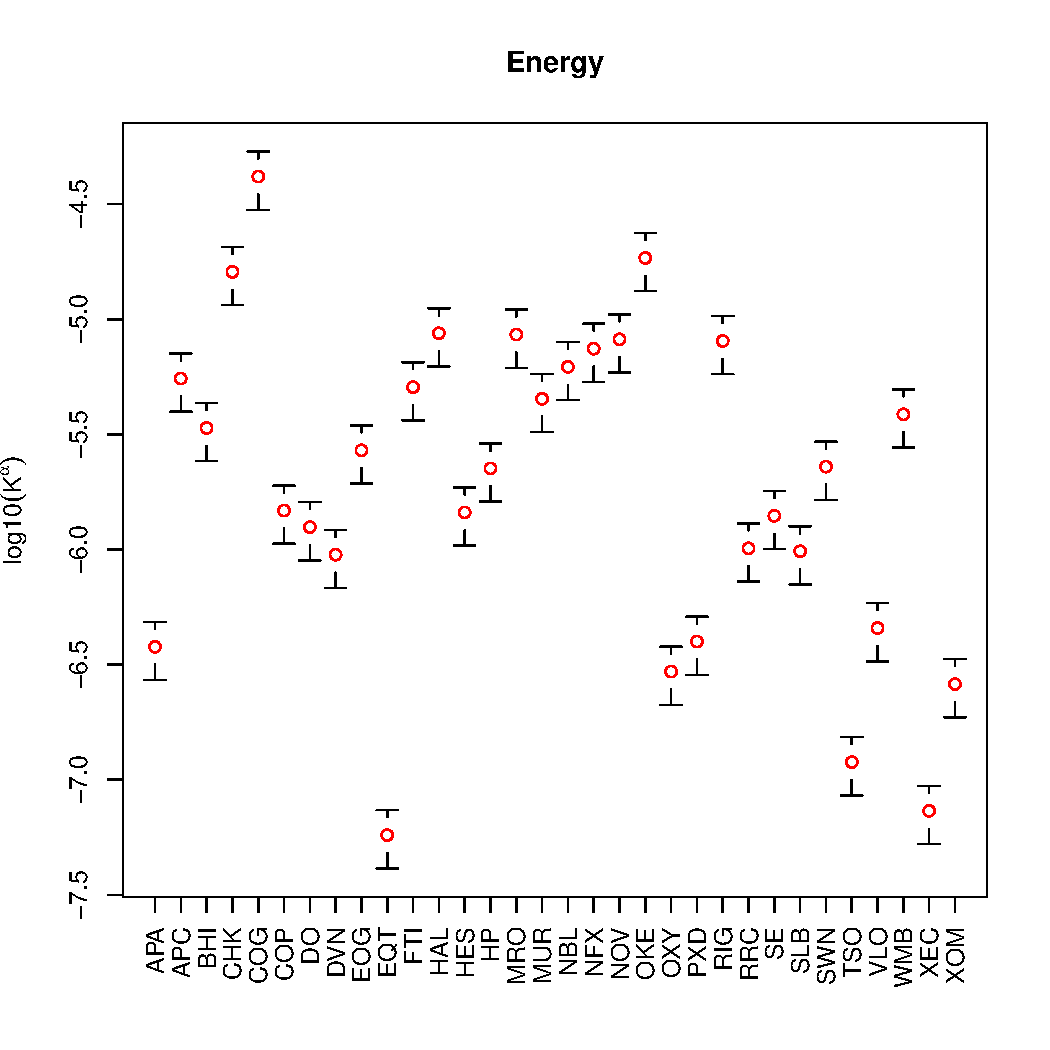
\includegraphics[width=\textwidth]
    {Energy_scale.pdf}
  \end{minipage}\hfill
  \begin{minipage}{0.33\linewidth}
    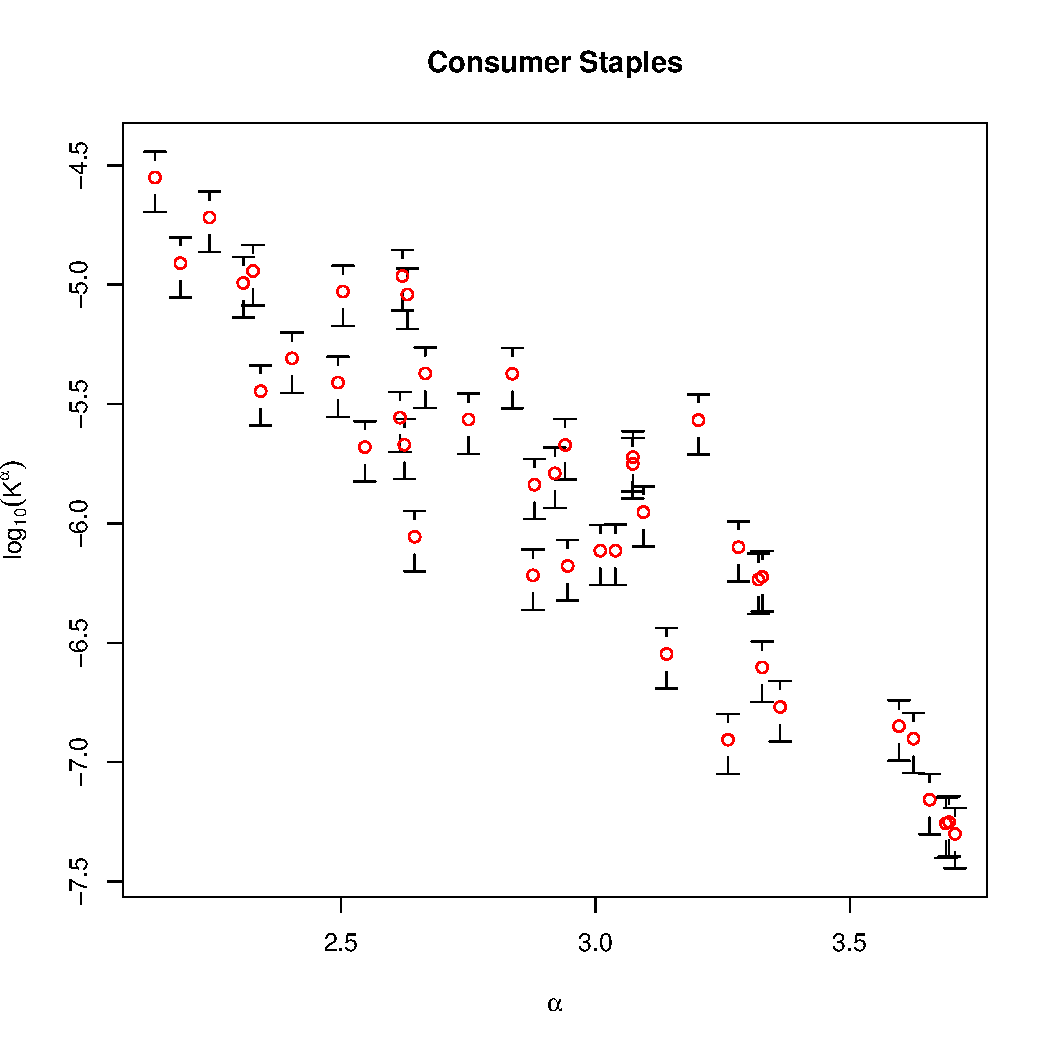
\includegraphics[width=\textwidth]
    {CS_scale.pdf}
  \end{minipage}\hfill
  \begin{minipage}{0.33\linewidth}
    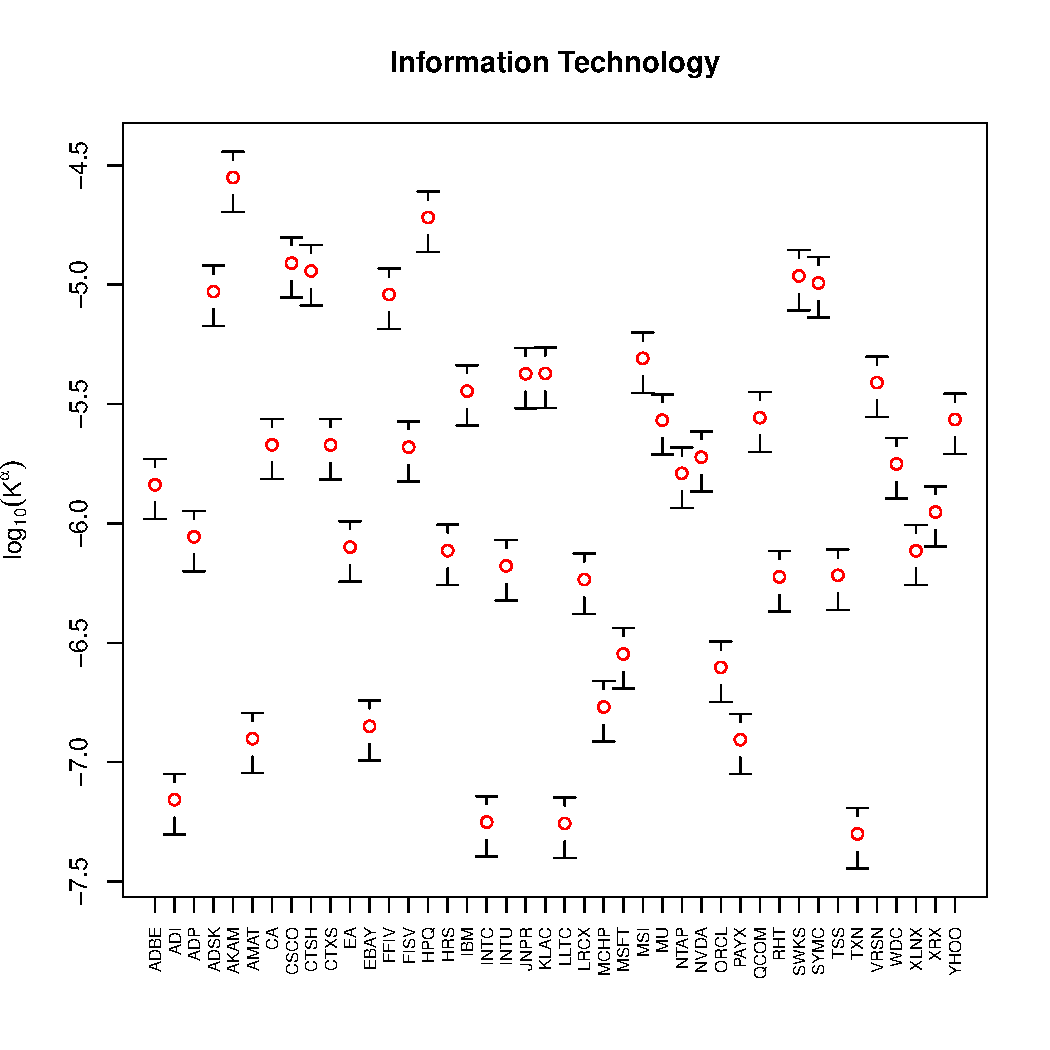
\includegraphics[width=\textwidth]
    {IT_scale.pdf}
  \end{minipage}
    \caption{\scriptsize Estimates of $\hat K_k$ (top) and
      $\hat K_k^{\hat \alpha}$ (bottom) on $\log_{10}$-scale.
      The bars are the asymptotic 95\%-confidence intervals.
    }
    \label{fig:sectors_parameters}
  \end{figure}
  \end{minipage}\hfill
  \begin{minipage}{0.35\linewidth}
    \begin{footnotesize}
      \begin{itemize}
      \item Estimated tail indices ($\hat \alpha$) and scale parameters
        $\hat K$ are positively dependent.
      \item The positive dependence is stronger for energy and IT stocks
        than for consumer staple's stocks.
      \item The scale $\hat K^{\hat \alpha}$ varies much more across different
        equities than does the tail index $\alpha$.
      \end{itemize}
    \end{footnotesize}
  \end{minipage}
\end{frame}

\begin{frame}
  \frametitle{Model of the market \& equity returns}
  \textcolor[HTML]{990033}{\bf The toy market consists of}
  \begin{enumerate}
  \item A riskless bond that pays $e^r$€ annually for each € invested,
    $r$ is fixed.
  \item A risky equity that pays $e^X$€ annually for each € invested.
    $X$ has Pareto tails
    \[
    F_X(x) = \left\{
      \begin{array}{ll}
        p \left(
          {K \over K - x}
        \right)^\alpha & x \leq 0 \,,\\
        1 - (1 - p) \left(
          {K' \over K' + x}
        \right)^\beta & x > 0\,,
      \end{array}
    \right.
    \]
  \end{enumerate}
\end{frame}

\begin{frame}
  \frametitle{Model of the investor}
  \begin{enumerate}
  \item He has 1 unit of currency for investment
  \item His happiness is proportional to a utility function $u(C)$:
    \begin{eqnarray*}
      C &=& (1 - \phi)e^r + \phi e^X \\
      u(C) &=& -C^{-\xi}/\xi, \quad \xi > 0 
    \end{eqnarray*}
    where
    \begin{itemize}
    \item $C$ is his monetary amount of consumption
    \item $\phi$ is the portion of his asset allocated to the equity
    \end{itemize}

  \item His preference over the equity is given by {\em
      Generalized Disappointment Aversion}:
    \[
    \tilde u (F_X, \phi) = \E u(C) - b \E [u(v) - u(C); C < v]
    \]
    where
    \begin{itemize}
    \item $v$ is the level of consumption below which
      the investor will be disappointed
    \item $b$ captures how disappointed the investor will be in case his consumption
      falls below $v$.
    \end{itemize}
  \end{enumerate}
\end{frame}

\begin{frame}
  \frametitle{Analytic results: when $\alpha$ and  $\beta$ are independent}
  \begin{minipage}[t]{0.5\linewidth}
    \begin{figure}[htb!]
      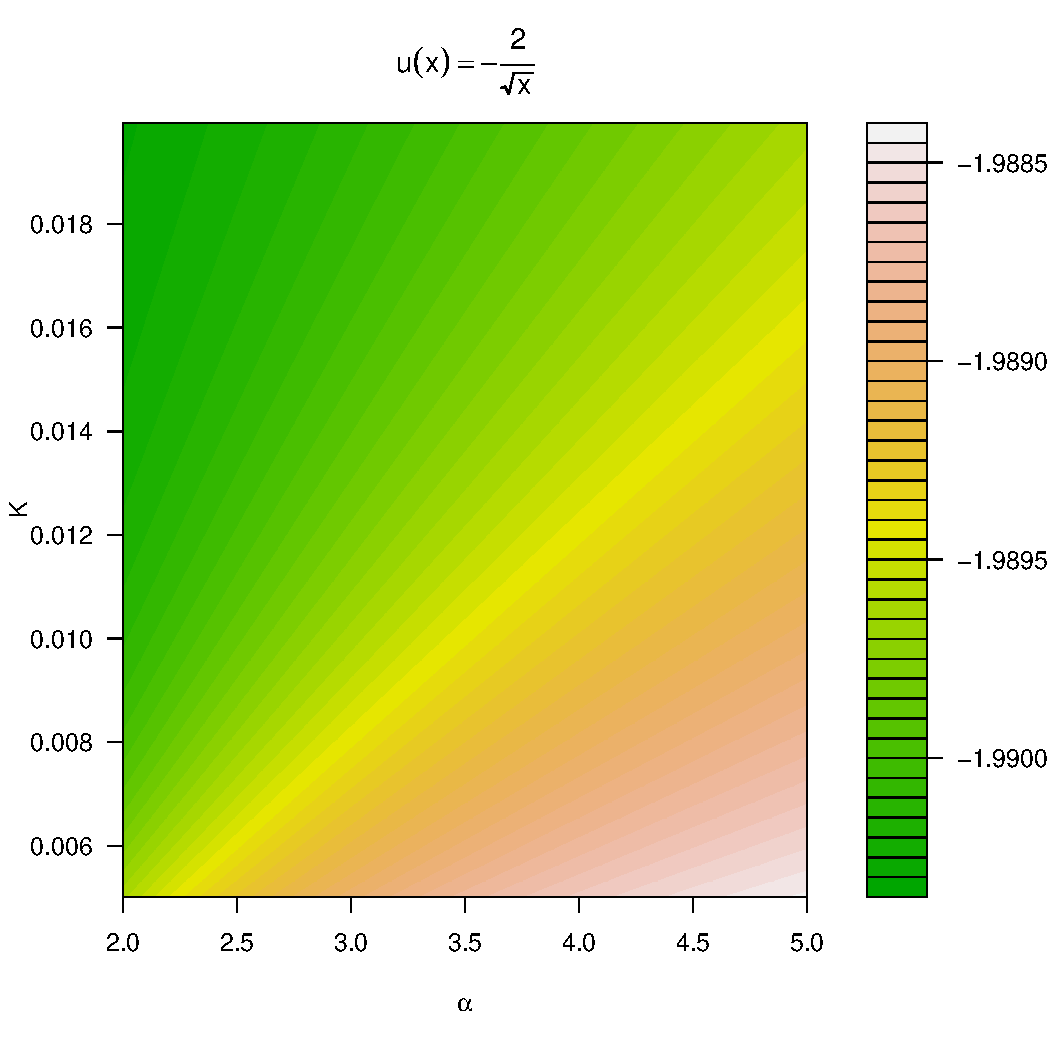
\includegraphics[width=\textwidth]{preference_pareto5e-1_A.pdf}
      \caption{\scriptsize
        $\tilde u_{\rm max}$ as a function of $\alpha$ and $K$
        in the two-sided Pareto model with $K'=0.012$, $\beta = 1.4$.
        $b = 0.01$ in all cases.
      }
    \end{figure}
  \end{minipage}\hfill
  \begin{minipage}[t]{0.5\linewidth}
    \begin{small}
      \begin{itemize}
      \item The investor's preference $\tilde u$ increases with $\alpha$ and
        decreases with $K$.
      \item Moving along a curve of equal preference, if $\alpha$
        increases then $K$ also increases.
      \item At market equilibrium, all actively traded stocks should
        have nearly the same investor preference -- $\alpha$ and
        $K$ values are expected to have positive dependence.
        % -- \textcolor[HTML]{990033}{\bf consistent with empirical results
        %   shown in figure \ref{fig:sectors_parameters}}.
        -- {\bf consistent with empirical results shown in figure
          \ref{fig:sectors_parameters}}.
      \end{itemize}
    \end{small}
  \end{minipage}
\end{frame}

\begin{frame}
  \frametitle{Analytic results: when $\alpha = \beta$}
  \begin{minipage}[t]{0.4\linewidth}
    \begin{figure}[htb!]
      \begin{minipage}{\linewidth}
        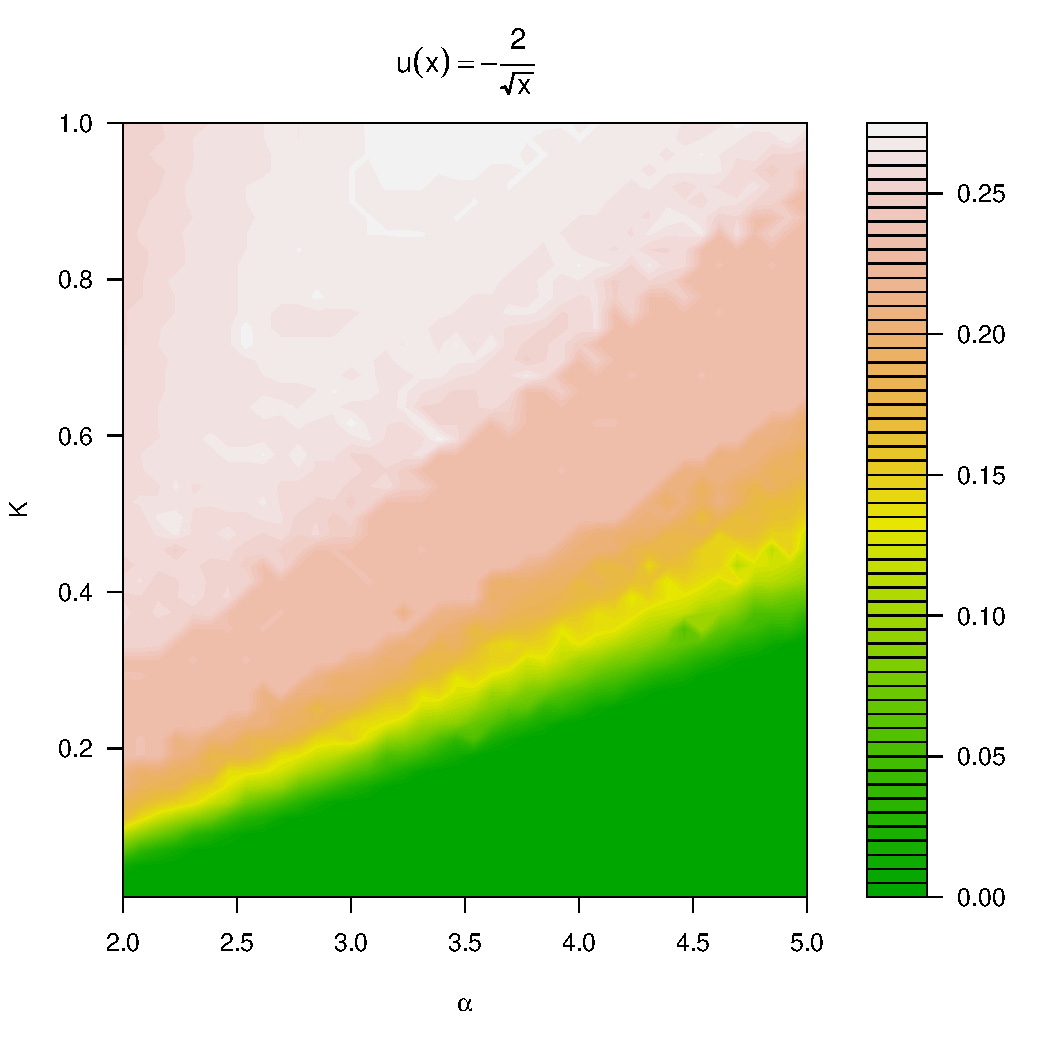
\includegraphics[width=1.0\textwidth, trim={0, 0, 0, 2cm}, clip]{phi_hat_pareto5e-1.pdf}    
      \end{minipage}\hfill
      \begin{minipage}{\linewidth}
        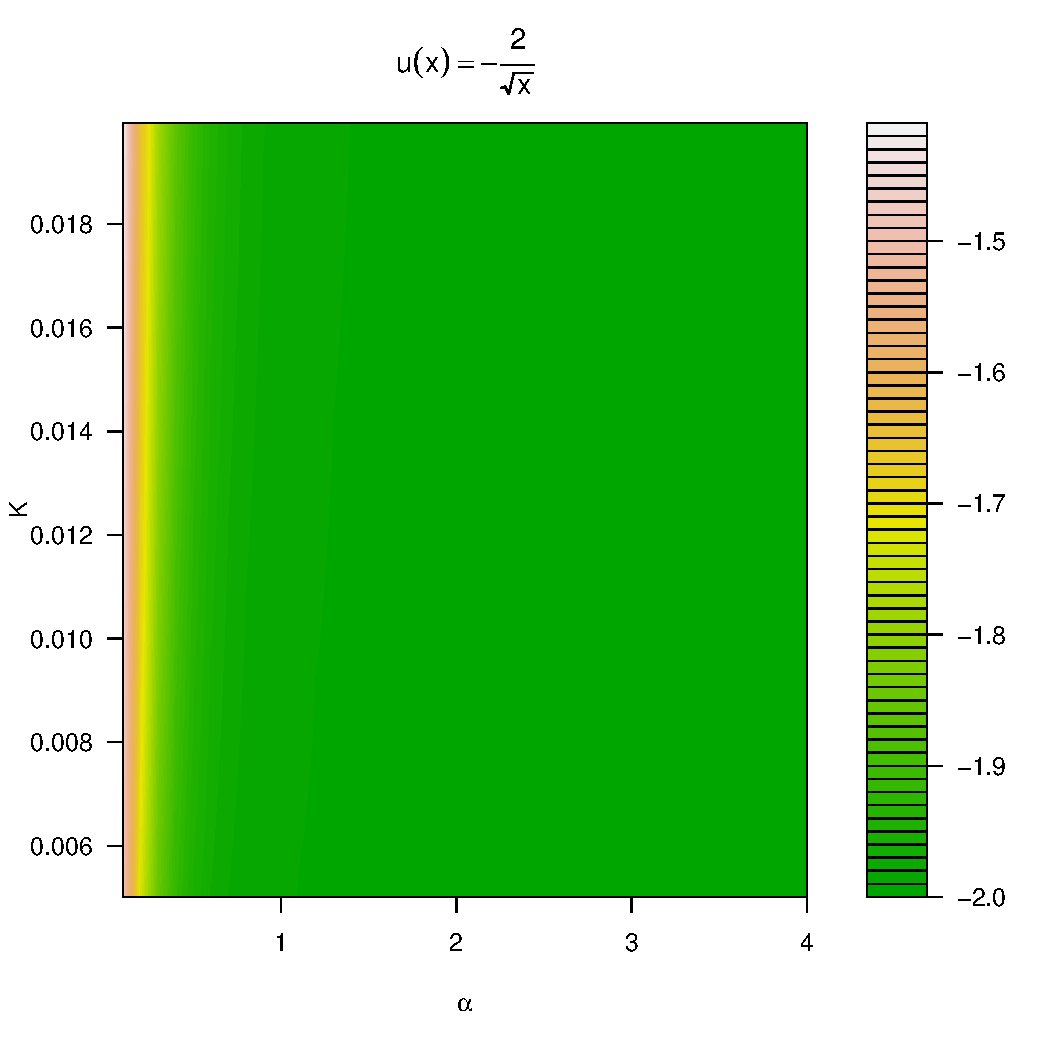
\includegraphics[width=1.0\textwidth, trim={0, 0, 0, 2cm}, clip]{preference_pareto5e-1.pdf}        
      \end{minipage}
    \end{figure}
  \end{minipage}\hfill
  \begin{minipage}[t]{0.6\linewidth}
    \begin{small}
      \textcolor[HTML]{990033}{\bf What's on the left?}
      \begin{itemize}
      \item Top: $\hat \phi(\alpha, K) = \argmax_{\phi} \tilde u(\alpha, K, \phi)$:
        optimal portion of allocation to the equity.
      \item Bottom: $\tilde u_{\rm max}(\alpha, K) = \max_{\phi} \tilde
        u(\alpha, K, \phi)$:
        Investor preference with optimal equity allocation.
      \item utility function $u(x) = -\frac{2}{\sqrt x}$
      \end{itemize}
      
      \textcolor[HTML]{990033}{\bf What I see from the plots}
      \begin{itemize}
      \item $\hat \phi$ is not monotone w.r.t. $\alpha$ or $K$.
      \item For a fixed $K$, $\hat \phi$ is decreasing with $\alpha$
        when $\alpha$ is in the range 2.5 $\sim$ 4.5, typical for real
        equity return series.
      \item $\tilde u_{\rm max}(\alpha, K)$ decreases with $\alpha$ 
        but is rather insensitive to $K$.
      \end{itemize}
    \end{small}
  \end{minipage}
\end{frame}

\begin{frame}
  \frametitle{When equity returns have t-distribution \& $b = 0$}
  The GDA preference reduces to {\em expected utility}. A few cases
  arise depending on
  \[
  a = {
    (1 - \phi) e^r
    \over
    \phi
  }, \quad
  y_\pm = {
    a^2 - \xi \pm \sqrt{(a^2 - 1) (a^2 - \xi^2)}
    \over
    a (\xi - 1)
  }
  \]
\begin{enumerate}
\item If $\max\{a, 1\} < \xi$, $\tilde u_{\rm max}$ is
  monotone increasing with $\alpha$.
\item If $a < \xi < 1$ and $(a + y_-)/(a y_- + 1) <
  y_-^{(1-\xi)/(1+\xi)}$, $\tilde u_{\rm max}$ is monotone
  increasing with $\alpha$.
\item If $\xi < a < 1$, $\tilde u_{\rm max}$ is monotone
  decreasing with $\alpha$.
\item If $1 < \xi < a$ and $(a + y_+)/(a y_+ + 1) >
  y_+^{(1-\xi)/(1+\xi)}$, $\tilde u_{\rm max}$ is monotone
  decreasing with $\alpha$.
\item In other case, $\tilde u_{\rm max}$ is not monotone
  w.r.t. $\alpha$.
\end{enumerate}
\end{frame}

\begin{frame}
  \frametitle{When equity returns have t-distribution \& $b > 0$}
  \begin{minipage}[t]{0.5\linewidth}
    \begin{figure}[htb!]
      \begin{minipage}{0.5\linewidth}
        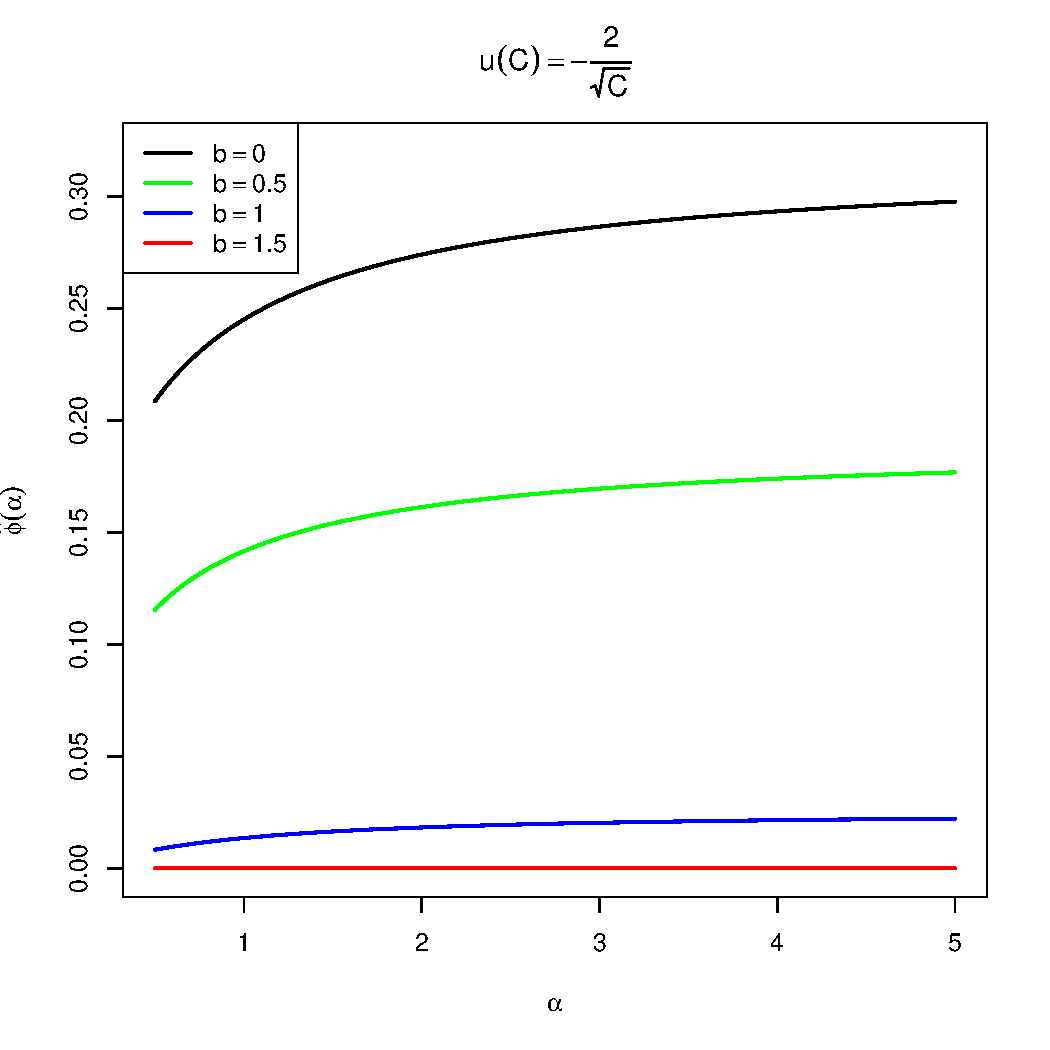
\includegraphics[width=\textwidth]{phi_hat_b_t_power.pdf}
      \end{minipage}\hfill
      \begin{minipage}{0.5\linewidth}
        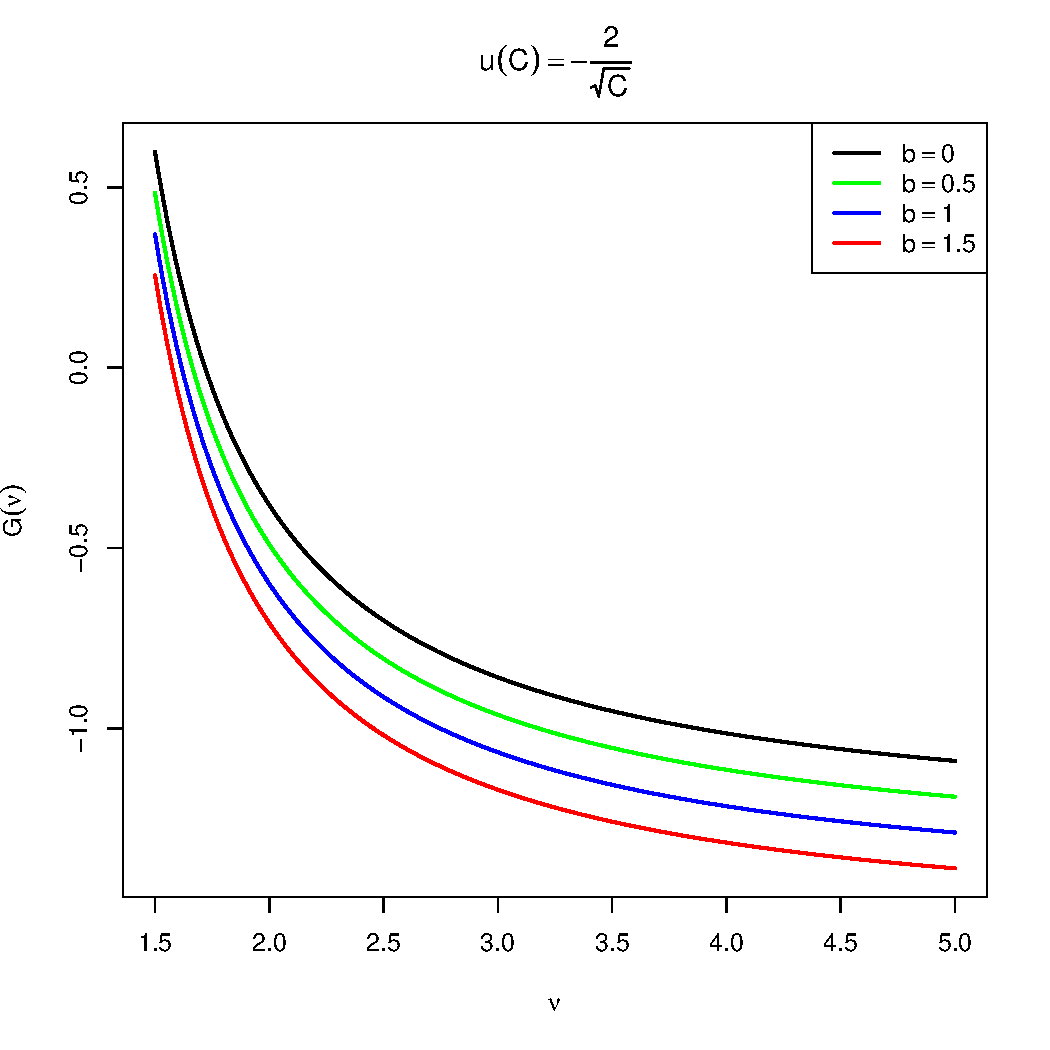
\includegraphics[width=\textwidth]{U_b_t_power.pdf}
      \end{minipage}
      \begin{minipage}{0.5\linewidth}
        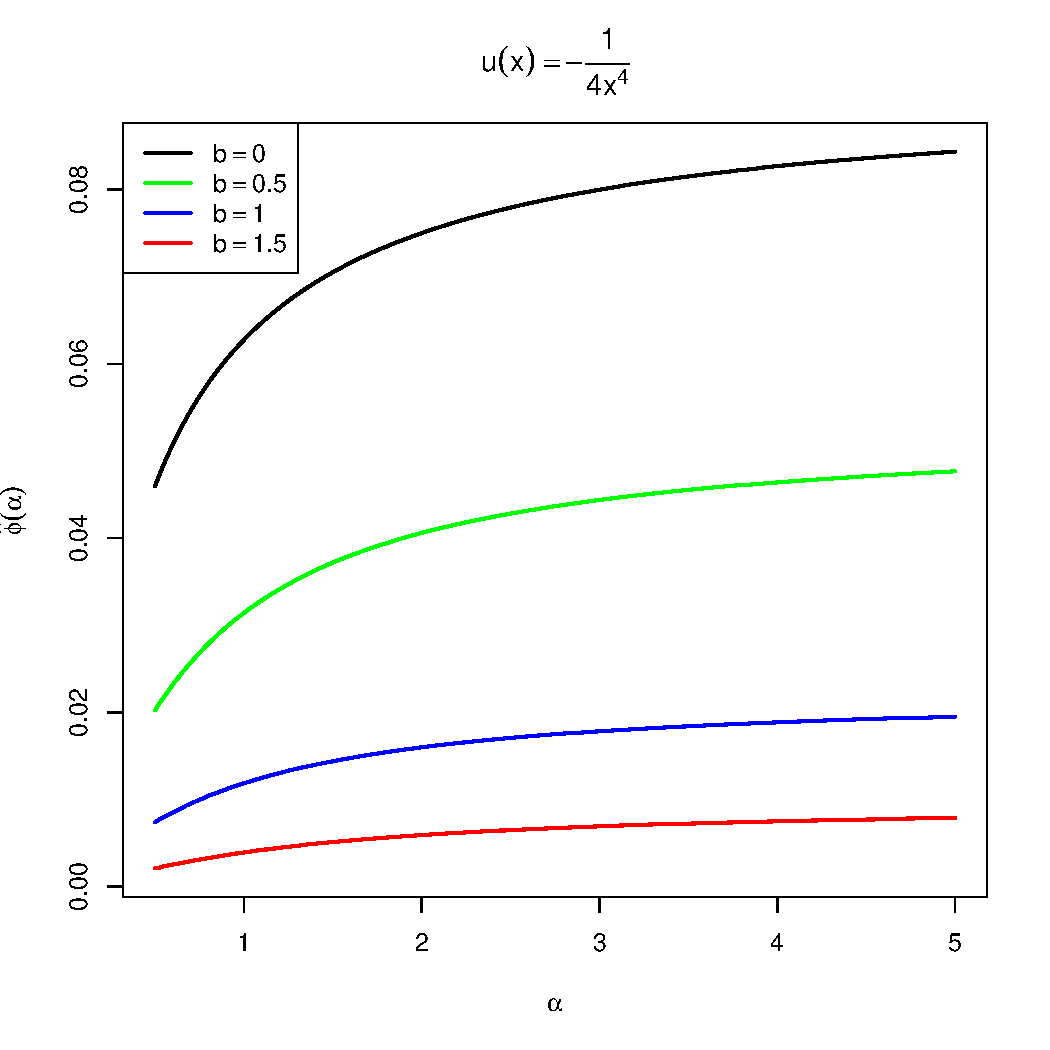
\includegraphics[width=\textwidth]{phi_hat_b_t_power4.pdf}
      \end{minipage}\hfill
      \begin{minipage}{0.5\linewidth}
        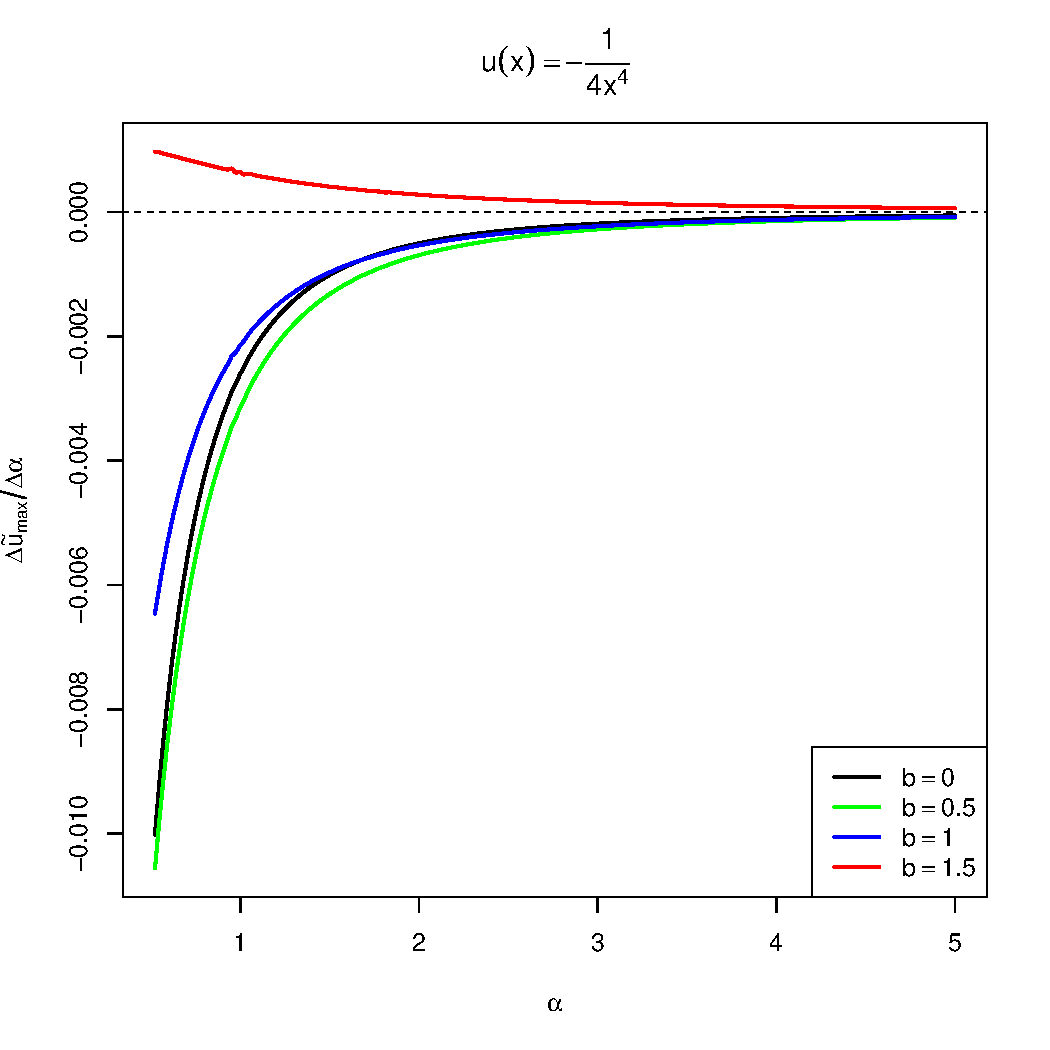
\includegraphics[width=\textwidth]{U_b_t_power4.pdf}
      \end{minipage}
      \caption{$\hat\phi$ (left) and
        ${\partial \tilde u_{\rm max} \over \partial \alpha}$ (right).
        {\em top:} $\xi = 1/2$. {\em bottom:} $\xi = 4$.
      }
      \label{fig:htfg}
    \end{figure}
  \end{minipage}\hfill
  \begin{minipage}[t]{0.5\linewidth}
    \textcolor[HTML]{990033}{\bf The figure says:}
    \begin{itemize}
    \item  $\hat\phi$ is monotone increasing for all 4 values of $b$
    \item $\tilde u_{\rm max}(\alpha)$ is increasing with $\alpha$
      when $b$ is relatively large, but  decreasing with $\alpha$ when
      $b$ is small
    \item A sizable value of $b$ indicates a conservative, risk-averse investor.
    \end{itemize}
  \end{minipage}
\end{frame}

\begin{frame}
  \frametitle{Summary}
  \begin{itemize}
  \item The tail index varies to different extent in different
    sectors/markets.
  \item The scale parameter is positively dependent on the tail index.
  \item The scale $K^{\alpha}$ varies much more across different
    equities than does the tail index $\alpha$.
  \item An investor's preference over $\alpha$ is dependent on the
    riskless rate of return, his own utility function and how
    disappointed he will be if his investment falls below
    expectation.
  \end{itemize}
\end{frame}

% \begin{frame}
%   \frametitle{Main ingredients of the derivation}
%   \begin{lemma} \label{lemma:I}
%     \begin{scriptsize}
%       Assume distribution function $F(x, \theta)$ parameterized by 
%       $\theta \in \Theta \subseteq \mathbb R$ has support
%       $(a, b) \subseteq \mathbb R$,
%       and in addition $F(x, \theta)$ has density
%       function $f(x, \theta)$ that is differentiable with respect to
%       $\theta$ for all $\theta \in \Theta$.
%       Let $X \sim F$ and assume function $h(\cdot)$ is defined on $(a, b)$
%       and is monotone throughout this interval.
%       Moreover, we assume $h(x)$ and $f(x, \theta)$ satisfy
%       \begin{equation}\label{eq:frt}
%         %    \E |h(X)| < \infty, \quad
%         \int_a^b \left| {\partial f(x, \theta) \over \partial \theta} \right| dx
%         < \infty \text { and }
%         \int_a^b \left| h(x) {\partial f(x, \theta) \over \partial \theta} \right| dx
%         < \infty
%       \end{equation}
%       Then the following holds true:
%       \begin{enumerate}
%       \item If $h(\cdot)$ is decreasing and $\exists x_0 \in (a, b)$ such that
%         $\frac{\partial f}{\partial \theta}(x, \theta) > 0$ for $x \in (a, x_0)$ while
%         $\frac{\partial f}{\partial \theta}(x, \theta) < 0$ for $x \in (x_0, b)$, then
%         \[
%         \frac{\partial \E h(X)}{\partial \theta} > 0
%         \]
%       \item If $h(\cdot)$ is increasing and $\exists x_0 \in (a, b)$ such that 
%         $\frac{\partial f}{\partial \theta}(x, \theta) < 0$ for $x \in (a, x_0)$  while
%         $\frac{\partial f}{\partial \theta}(x, \theta) > 0$ for $x \in (x_0, b)$, then
%         \[
%         \frac{\partial \E h(X)}{\partial \theta} > 0
%         \]
%       \end{enumerate}
%     \end{scriptsize}
%   \end{lemma}
% \end{frame}

% \begin{frame}
%   \frametitle{Proof}
%   \begin{scriptsize}
%     We prove it in the first case. The other case is similar.
%     By dominated convergence theorem, conditions \eqref{eq:frt}
%     imply, for all $S \subseteq (a, b)$,
%     \begin{eqnarray*}
%       {\partial \over \partial \theta}\int_S f(x, \theta) dx
%       &=&
%       \int_S {\partial \over \partial \theta} f(x, \theta) dx \\
%           {\partial \over \partial \theta}\int_S h(x) f(x, \theta) dx
%           &=&
%           \int_S h(x) {\partial \over \partial \theta} f(x, \theta) dx \\
%     \end{eqnarray*}
%     Thus we have
%     \begin{eqnarray*}
%       {\partial \E h(X) \over \partial \theta}
%       &=&
%       {\partial \over \partial \theta}
%       \int_a^b h(x)
%       f(x, \theta) dx \\
%       &=& \int_a^b h(x)
%       {\partial f \over \partial \theta}(x, \theta) dx \\
%       &=& \underbrace{\int_a^{x_0}
%         h(x) {\partial f \over \partial \theta}(x, \theta) dx}_{I_1}
%       + \underbrace{\int_{x_0}^b
%         h(x) {\partial f \over \partial \theta}(x,
%         \theta) dx}_{I_2}
%     \end{eqnarray*}
%   \end{scriptsize}
% \end{frame}

% \begin{frame}
%   \frametitle{Proof cont'd}
%   \begin{scriptsize}
%     $x_0$ being located in the interior of $(a, b)$ and
%     $h(\cdot)$ being monotone imply $h(x_0) < \infty$.
%     When $h(x)$ is decreasing on $(a, b)$ and
%     ${\partial f \over \partial \theta}(x, \theta) > 0$ on $(a, x_0)$
%     \[
%     I_1 > h(x_0) \int_a^{x_0}
%     {\partial f \over \partial \theta}(x, \theta) dx
%     \]
%     Similarly, because
%     ${\partial f \over \partial \theta}(x, \theta) < 0$ for
%     $x \in (x_0, b)$ and $h(x)$ is decreasing, we have
%     \begin{eqnarray*}
%       I_2 &=& \int_{x_0}^b -h(x_0)
%       \left|{\partial f \over \partial \theta}(x, \theta) \right| dx
%       > -h(x_0)
%       \int_{x_0}^b \left| 
%           {\partial f \over \partial \theta}(x, \theta)
%           \right| dx
%     \end{eqnarray*}
%     Finally we have
%     \begin{eqnarray*}
%       {\partial \E h(X) \over \partial \theta}
%       > h(x_0) \int_a^b
%       {\partial f \over \partial \theta}(x, \theta) dx
%       = h(x_0) {\partial \over \partial \theta}
%       \int_a^b f(x, \theta) dx
%       = 0
%     \end{eqnarray*}
%   \end{scriptsize}
% \end{frame}

\begin{frame}
   \frametitle{Thank you!}
   Questions?
 \end{frame}
\bibliographystyle{unsrt}
\bibliography{../../thesis/econophysics}
\end{document} 
